\documentclass[11pt,letterpaper]{article}
\usepackage[T1]{fontenc}
\usepackage[margin=1in]{geometry}
\usepackage{array}
\usepackage{booktabs}
\usepackage{longtable}
\usepackage{microtype}
\usepackage{tabularx}
\usepackage{tikz}
\usetikzlibrary{positioning,fit,arrows.meta,shapes.geometric}
\usepackage[hidelinks]{hyperref}
\usepackage[nameinlink,noabbrev]{cleveref}
\usepackage[numbers,sort&compress]{natbib}

% Keep the manuscript buildable with a portable pdflatex toolchain.
% A venue-specific build may replace this lightweight natbib bibliography.
\newcommand{\parencite}[1]{\citep{#1}}
\setlength{\parindent}{0pt}
\setlength{\parskip}{0.55\baselineskip}
\setlength{\tabcolsep}{3pt}
\setlength{\emergencystretch}{1.5em}
\newcolumntype{P}[1]{>{\raggedright\arraybackslash}p{#1}}

\title{Cross-Layer Alignment in the Human-Agent Enterprise}
\author{James Booth}
\date{23 October 2026}

\begin{document}
\maketitle

\begin{abstract}
Enterprise agents can interpret requests, use tools, and coordinate work, but useful execution depends on organizational conditions that are maintained outside the agent runtime. Ontologies help establish meaning; identity and policy systems constrain authority; process models describe allowable work; enterprise architecture connects capabilities to objectives. None of these representations alone establishes whether a delegated action remains appropriate as responsibilities, process state, data, and permissions change. This paper develops a structured interdisciplinary synthesis of \emph{cross-layer alignment}: evidence-supported correspondence among semantic, structural, process, and strategic representations under cross-cutting governance. It clarifies the difference between knowing an enterprise rule, being authorized to act, and observing the result. Two compound scenarios illustrate why a locally valid tool call can conflict with broader organizational conditions. We discuss context freshness, multi-level delegation, data provenance, and runtime evidence as design considerations, including situations where adversarial or automated changes may outpace human review. The paper proposes a bounded architectural vocabulary and research questions, not a validated security architecture, numerical alignment score, or empirical claim of improved outcomes.
\end{abstract}

\section{Introduction}
An enterprise agent acts through a web of concepts, actors, processes, permissions, and objectives. A customer case may be represented in a semantic model, owned by a service team, routed through an exception-aware process, constrained by a policy service, and evaluated against a strategic objective. These representations can disagree even when each is locally plausible. A vocabulary can be correct while an agent is assigned to the wrong role. A process can be conformant while a tool call exceeds authority. An organizational chart can be accurate while the event data omit the informal escalation that makes the work safe.

This paper asks how to study that consistency problem without overstating what adjacent research has already achieved. Agentic Business Process Management (Agentic BPM) is now a substantial research stream. The AI-augmented BPM systems manifesto described framed autonomy, sensing, reasoning, explanation, adaptation, and improvement in process-aware systems \parencite{dumas2023abpms}. Recent Agentic BPM work makes process frames, goals, normative constraints, human and software agents, and process mining more explicit \parencite{calvanese2025normative,calvanese2026manifesto,dumas2026abpms}. Formal foundations further treat agents as goal-directed decision makers operating under strategies and guardrails \parencite{degiacomo2026formal}. Any claim that the literature has not connected agents, processes, goals, and governance would therefore be inaccurate.

The narrower question is whether the literature provides a common conceptual object for the consistency relations among several enterprise layers: semantic meaning; actor and team topology; prescribed and observed process; strategic intent and architecture; and governance constraints on delegation and action. The distinction matters because a process-aware agent can still use ambiguous concepts, inherit an observed-but-unauthorized topology, encounter tacit exceptions, or operate under permissions that do not match the process or intended risk posture.

The paper is a structured interdisciplinary conceptual synthesis and perspective paper. Its purpose is to explain how enterprise architecture and organizational knowledge relate to agent execution, rather than merely list properties a well-designed agent should have. It does not estimate alignment prevalence, establish causal effects, or validate an enforcement architecture. The central object is cross-layer alignment: evidence-supported correspondence, compatibility, or productive coordination among representations relevant to a bounded delegated action. The negative case is cross-layer mismatch; insufficient or untrusted evidence remains a separate condition. A semantically coherent plan is not an authorization decision, and a permitted tool invocation is not proof that the resulting business action was correct.

The architectural implication is that relevant context must be discoverable, attributable, sufficiently current for the action, and available to independent controls at execution boundaries. Changes are not uniformly fast. Ownership and strategy can change on human time scales, while credentials, incident state, workload identity, data flows, and adversarial activity can change on automated time scales. An enterprise cannot assume its control and revalidation loop has the same reaction window as a human approval workflow. This is a prospective design requirement, not a measured claim that every enterprise process is already machine-speed.

The paper makes five contributions:

\begin{enumerate}
\item It develops a cross-layer framing for an organizational design problem while explicitly crediting Agentic BPM, DEMO, semantic BPM, Human--AI Teaming, and Digital Twin research for important partial combinations.
\item It provides a vocabulary that keeps semantic foundation, actor topology, process representation, strategic intent and architecture, and governance constraints analytically distinct.
\item It identifies recurring cross-layer mismatch patterns and explains how prescribed, observed, authorized, and effective representations can diverge.
\item It organizes each dimension around working definitions, relevant representations, evidence sources, possible misalignment, consequences, and confounders.
\item It proposes an empirical research agenda for testing construct usefulness, observable indicators, inter-rater reliability, outcome association, interaction, and boundary conditions.
\end{enumerate}

\section{Research Method and Scope}
\subsection{Structured interdisciplinary conceptual synthesis}
The synthesis was designed to challenge, refine, and situate a cross-layer alignment construct rather than to estimate prevalence or perform a statistical meta-analysis. The principal search and chaining process was conducted through 31 August 2026, with a targeted update through 23 October 2026 on runtime authorization, multi-agent delegation, Zero Trust, organizational context, and agent observability. It combined targeted searches, citation chaining, and source inspection across the following domains: semantic interoperability, enterprise ontology, semantic BPM, Human--AI and Human--Autonomy Teaming, multi-agent systems, process mining, Agentic BPM, governance and authorization, enterprise architecture, and Digital Twins of Organizations.

Search terms combined variants of "human-agent enterprise," "cross-layer alignment," "organizational alignment," "semantic interoperability," "actor topology," "human-AI teaming," "delegation," "autonomy boundaries," "process mining," "Agentic BPM," "organizational mining," "agent identity," "authorization," "enterprise architecture," and "digital twin of organization." Inclusion favored sources that defined relevant constructs, supplied a process or organizational representation, reported empirical observations, described governance mechanisms, or provided a useful conceptual bridge. Exclusion favored duplicate versions, sources without recoverable metadata, purely promotional material, and work whose relation to enterprise action could not be established.

The corpus intentionally combines foundational books and papers, standards, peer-reviewed journal and conference work, practitioner and governance documents, and recent preprints. Foundational sources establish vocabulary or representational traditions; recent sources expose current Agentic BPM, teaming, governance, and organizational-mining developments. Practitioner documents and standards are used for design context rather than counted as causal evidence. Citation chaining was used to locate adjacent work and test the initial framing against related perspectives. The targeted October update adds standards and technical guidance alongside recently published research, with document status identified where relevant. The resulting synthesis is purposive and auditable, not exhaustive.

\subsection{Evidence categories and auditability}
Evidence labels in this paper are descriptive synthesis labels, not confidence levels, systematic-review grades, or meta-analytic estimates. "Strong direct" indicates that a source studies a closely matching construct and outcome in a relevant setting. "Emerging direct" indicates a close but early or bounded study. "Strong adjacent" indicates a well-supported neighboring mechanism. "Conceptual / speculative" indicates a reasoned integration or research proposition that still requires direct testing. These labels communicate what kind of support a claim has; they do not assign numeric certainty.

\section{Background and Terminology}
\subsection{Semantic foundation is not one artifact}
Semantic interoperability is the ability of independently produced systems, people, or agents to interpret exchanged concepts consistently enough for an intended task. It includes more than matching labels: entity identity, context, constraints, provenance, versioning, and exception interpretation matter. Retrieval augmentation and knowledge-graph integration can improve grounding in bounded tasks, but grounding quality depends on coverage, freshness, retrieval, entity resolution, and evaluation design \parencite{lewis2020retrieval,pan2024unifying}.

An ontology is a formal specification of categories, relations, constraints, and an intended conceptualization \parencite{gruber1993translation,guarino1998formal}. A knowledge graph is a graph-shaped representation of entities, relationships, and assertions; it may use an ontology or schema but is not equivalent to one. A semantic model is an umbrella term for a representation that gives data or process artifacts interpretable meaning and relationships. A semantic layer is an implementation-facing or business-facing abstraction that maps raw structures and metrics to governed business concepts. A taxonomy is a hierarchy or controlled classification, while a schema primarily specifies structure, fields, and allowable shapes. OWL and SKOS illustrate distinct standards roles in formal semantics and controlled vocabularies \parencite{w3cowl2004,w3cskos2009}. Keeping these terms separate prevents the presence of a graph, vocabulary, or schema from being treated as evidence that an agent has the intended meaning.

\subsection{Actors, roles, topology, and delegation}
Actor topology describes the structure of actors and their organizational relationships relevant to execution and governance of work. It includes actor identity and type, role assignment, responsibility boundaries, authority and delegation relationships, interaction and communication relationships, autonomy limits, and interfaces between human, agent, and system actors. It is a boundary object connecting organization design, team configuration, process execution, and software architecture; it is not synonymous with an organizational chart or a network diagram.

The construct distinguishes actor, team, role, responsibility, authority, delegation, autonomy, interaction, interface, and organizational or software boundary. A role is an expected position or pattern of participation; responsibility concerns what an actor is answerable for; authority concerns which actions or decisions an actor may take; delegation transfers bounded authority; autonomy concerns the latitude to select or execute actions within those bounds. These distinctions matter when a system can perform an action technically but is not authorized to perform it, or when a human remains accountable after an agent has executed a delegated step.

For a bounded work domain, topology should be examined in at least four versions. The prescribed topology describes intended assignments and relationships. The observed topology describes interactions and participation recovered from event data, communication records, or other observations. The authorized topology describes identities, permissions, delegation paths, and governance-approved relationships. The effective topology describes what actually shaped execution in context, including informal work, tacit escalation, and runtime substitutions. These versions can agree, conflict, or remain only partially observed. Agent Miner and organizational mining show that aspects of agent systems and interactions can be recovered from event data, while Human--AI Teaming work shows that role structure, interdependence, leadership, communication, and team lifespan change team behavior \parencite{tour2023agentminer,orgmining2026,verhagen2024trust,hughes2026teams}.

\subsection{Process, strategy, and governance}
A process representation describes prescribed or intended work, including states, activities, events, decisions, dependencies, actors, data, and exception paths. Event data provide an observation of enacted work, not a complete account of work. BPMN, DEMO, process mining, and Agentic BPM therefore address related but non-identical views of process meaning and execution \parencite{dietz2006enterprise,omg2014bpmn,aalst2016process,dumas2023abpms}.

Strategic intent concerns objectives, capabilities, priorities, risk appetite, and the reasons an organization authorizes a class of work. Enterprise architecture provides representations of capabilities, organization, applications, services, data, and dependencies through different viewpoints \parencite{zachman1987framework,togaf2022standard,archimate2022standard}. Governance is the cross-cutting constraint plane that determines which actions, relationships, states, and delegations are permissible and how they are monitored, attributed, interrupted, revoked, and reviewed. It includes identity, permission, prohibition, obligation, delegation, approval, separation of duties, monitoring, attribution, audit, revocation, interruptibility, and autonomy boundaries. Other literatures may classify governance as a capability or pillar; this paper uses the constraint-plane view to emphasize its effects across all dimensions.

\subsection{Bounded delegation, tacit knowledge, and epistemic status}
For a delegated action, the relevant knowledge may be explicit in a policy, process model, schema, or authorization record; observed in event data or runtime traces; inferable from governed evidence; or tacit, contested, or absent from machine-accessible representations. Research on tacit knowing and organizational knowledge creation cautions that practical judgment and socially transmitted context cannot be assumed to be fully captured by formal records \parencite{polanyi1966tacit,nonaka1995knowledge}. Bounded delegation requires the organization to specify the action boundary, the responsible and authorized actors, the process context, applicable constraints, escalation path, monitoring, attribution, and revocation or interruption conditions. The importance of each element varies with task reversibility, impact, exception rate, and regulatory or operational exposure. This paper does not assume a fixed functional relationship among these elements.

The following epistemic distinctions are essential:

\begin{description}
\item[Alignment] Available evidence indicates that the relevant representations agree or are compatible for the bounded task.
\item[Misalignment] Available evidence indicates that relevant representations conflict, omit a required constraint, or authorize and enact incompatible behavior.
\item[Unknown or insufficient evidence] Available evidence is too incomplete, stale, ambiguous, or contradictory to determine whether the representations agree.
\end{description}

Poor observability is not automatically misalignment. It is an evidence limitation that may increase uncertainty, reduce the defensible autonomy boundary, or motivate additional instrumentation and human review. Similarly, a difference between prescribed and effective practice can be intentional adaptation, a benign local variation, a governance breach, or simply an unobserved explanation; classification depends on context and evidence.

\section{Related Work}
\subsection{Semantic foundations and semantic BPM}
Enterprise ontology, formal ontology, semantic Web standards, semantic BPM, and BPMN semantics provide established foundations for shared meaning and executable process descriptions \parencite{gruber1993translation,guarino1998formal,hepp2005semantic,annane2019bbo}. Knowledge graphs, retrieval augmentation, and neuro-symbolic approaches offer mechanisms for grounding, querying, constraint checking, and provenance \parencite{lewis2020retrieval,pan2024unifying,sarker2021neuro}. Their boundary for this paper is not weakness in semantic representation; it is that semantic validity does not settle actor responsibility, authority, strategic priority, or tacit exception handling.

\subsection{Organizational and actor topology}
Organization design and software architecture research has long connected communication structure, responsibility, and system boundaries. Conway's law and the mirroring literature motivate attention to correspondence between organizational and technical structures \parencite{conway1968committees,macCormack2012exploring}. Team Topologies makes team boundaries, interaction modes, and cognitive load operationally salient \parencite{skelton2019team}. Multi-agent systems provide mature abstractions for autonomous actors and coordination, but often abstract away institutional semantics and enterprise authority \parencite{wooldridge1995intelligent,dorri2018multiagent}. Agent Miner and organizational mining add data-driven routes for discovering agent types and interaction structures from event data \parencite{tour2023agentminer,orgmining2026}.

\subsection{Human--AI and Human--Autonomy Teaming}
Human--AI and Human--Autonomy Teaming provide direct evidence that agents are not merely tools in every operating configuration. Shared mental models concern the similarity and adequacy of team members' representations of tasks and other members \parencite{andrews2022smm}. Reviews of AI teaming connect team constellation, trust, shared cognition, coordination, and mutual understanding, and warn that poor team cognition can reduce performance \parencite{schmutz2024aiteaming}. An experiment with 80 participants found that task interdependence affected the relation between perceived trust and system trustworthiness \parencite{verhagen2024trust}. Other controlled work links agent status and task conditions to trust and blame \parencite{gall2024trust}.

Recent reviews make topology more specific. A systematic review of Human--Agent Teaming and multi-agent interactions discusses task allocation, workload, resilience, trust, and differences between single-agent and multi-agent teams \parencite{yu2025hat}. A trust-assessment review separates subjective and objective measures and identifies gaps in dynamic and distributed teams \parencite{jahan2025trust}. A 2026 scoping review of experimental papers identifies clusters of teaming configurations and records task interdependence, roles, leadership, communication, distribution, and lifespan \parencite{hughes2026teams}. A proceedings abstract proposes a multi-dimension typology based on review and expert input \parencite{engelhardt2026typology}. These findings support topology as a useful analytical dimension and contradict any assumption that human--AI team denotes one stable configuration.

Mixed-initiative work treats initiative as bi-directional and adaptive, with capability, reliance, communication, and task context changing over time \parencite{natarajan2025mixed}. Organizational reviews connect human--AI collaboration to trustworthiness, organizational needs, and testable relationships \parencite{dokhac2026hai}. The literature motivates observables such as handoff latency, escalation appropriateness, supervision load, authority clarity, shared-mental-model indicators, calibrated reliance, accountability attribution, and human workload. It does not yet establish a general mapping from those constructs to enterprise ontology, process conformance, system architecture, and delegated authority.

\subsection{Multi-agent systems, process mining, and Agentic BPM}
Process mining supplies an observable substrate for comparing prescribed and enacted work. Agent Miner discovers agent interaction models from event data and reports evaluation on public industrial datasets \parencite{tour2023agentminer}. Organizational mining extends this direction with agent types and interactions evaluated through precision, recall, simplicity, and modularity \parencite{orgmining2026}. Process records have also been used to generate project-specific AI-agent roles in bounded software-engineering settings, with functional tests and exploratory user evidence \parencite{bala2026agents}. These methods make observed topology and process variation more inspectable; they do not by themselves establish authorized topology, semantic agreement, or strategic alignment.

Agentic BPM is the closest adjacent stream. The 2023 ABPMS manifesto frames sensing, reasoning, acting, explaining, adapting, and improving within process-aware systems \parencite{dumas2023abpms}. Later work makes goals and normative frames first-class, proposes Agentic BPMS architectures, develops formal foundations, and articulates a broader research manifesto \parencite{calvanese2025normative,dumas2026abpms,degiacomo2026formal,calvanese2026manifesto}. A practitioner-interview synthesis also documents concerns about data inconsistency, manual intervention, transparency, and governance; its findings motivate questions rather than establish generalized outcomes \parencite{vu2025agentic}. These streams already combine important elements. Building from that work, this paper asks how to compare the consistency of semantic, topological, process, strategic, and governance representations across those systems, and how to test whether such comparison is useful.

\subsection{Governance, authorization, and bounded autonomy}
Governance work emphasizes layered controls, human oversight, monitoring, attribution, escalation, and interruption \parencite{shavit2023governance,schmitz2025oversight}. Recent autonomy-level proposals distinguish what an agent can technically do from what it is permitted to do \parencite{zheng2026permission}. NIST's draft agent identity and authorization concept paper likewise discusses verifiable identity, authorization, and lifecycle controls as considerations for trustworthy deployment \parencite{nist2026identity}. These sources support governance as a cross-cutting constraint plane. They do not imply that a governance record is complete, current, or aligned with process practice, organizational responsibility, or strategic intent.

\subsection{Zero Trust, policy enforcement, and organizational context}
Established Zero Trust work removes implicit trust based on location or ownership and places access decisions at identity-aware application and service boundaries. NIST SP 800-207A describes gateways, workload identities, and sidecars for granular enforcement; OPA documentation provides a concrete pattern in which an agent harness consults an independent policy decision point (PDP) before executing a tool call \parencite{nist207a2023,opa2026agent}. These mechanisms do not themselves establish whether an input attribute reflects the applicable organizational meaning, accountable owner, process version, or permissible business purpose. An authorization system needs authoritative contextual inputs; the agent's own explanation cannot be accepted as a grant of authority.

J{\o}rgensen and Ma's 2026 bounded-autonomy framework is particularly close: it separates agent proposals from independently validated semantic meaning, process admissibility, organizational authority, controlled execution, and provenance \parencite{jorgensen2026governing}. The present synthesis does not claim to invent that separation. A more specific question remains about maintaining consistency when agents are created and destroyed dynamically, authority is delegated across several hops, contextual attributes change during execution, and information is combined across authorized inputs. Tallam identifies transitive delegation, aggregation inference, and temporal validity as connected authorization-propagation problems \parencite{tallam2026authorization}. Recent organizational-context work similarly emphasizes the need to detect when assertions from human-authored sources become stale relative to live state \parencite{yavin2026context}.

\subsection{Dynamic agent teams and operational evidence}
Temporary or dynamically created sub-agents allow task decomposition and parallel work but do not replace every persistent or role-specific agent. A recent preprint comparing dynamic concurrency on coding tasks reports conditional benefits alongside coordination failures and increased execution cost; it does not establish universal superiority or enterprise-scale performance \parencite{li2026subagents}. Multi-agent Zero Trust work already studies mission-scoped authority, independently enforced tool access, and adversarial cooperation in simulated response settings \parencite{chen2026swarmgov}. This paper treats dynamically changing actor topology as a demanding example through which the cross-layer problem becomes visible, reserving protocol design and comparative evaluation for subsequent research.

The W3C PROV ontology supplies transferable terms for entities, activities, agents, derivation, attribution, and delegation, while emerging OpenTelemetry conventions instrument agent creation, invocation, planning, and tool execution \parencite{w3c2013prov,otel2026agent}. These are useful evidence substrates but not proof of authorization or business alignment. In particular, content-rich prompts and traces can expose sensitive information; adequate evidence must be captured with proportionate retention, access control, and data minimization.

\subsection{Enterprise architecture and Digital Twins of Organizations}
Enterprise architecture frameworks supply traceability among strategy, capabilities, organization, systems, and information \parencite{zachman1987framework,togaf2022standard,archimate2022standard}. Digital Twins of Organizations (DTOs) extend the digital-twin idea toward organizational structures, processes, event traces, constraints, and action-oriented feedback \parencite{park2021dto,lyytinen2024dto}. Work on organization design argues that DTOs can reshape how organizational arrangements are represented and examined \parencite{lyytinen2024dto}. Agentic digital-twin demonstrations connect agent interfaces to operational data \parencite{timms2025digitaltwin}. The present paper treats DTO as an optional evidence substrate for linking partial representations, not as a new DTO architecture or as a guarantee of organizational knowledge.

\section{Cross-Literature Intersections}
The literatures intersect around a recurring practical situation: multiple representations are individually useful but jointly inconsistent or incomplete. Semantic BPM can connect concepts to process steps without settling which human or software actor may perform them. HAT research can characterize trust, roles, interdependence, and workload without tracing those constructs to enterprise policy or architecture. Process mining can expose enacted variants without establishing whether the variants are authorized or strategically intended. Enterprise architecture can trace capabilities and ownership without observing runtime handoffs. Governance can define permissions and approvals without proving that the process model, actor topology, semantic layer, and effective behavior agree.

This intersection suggests four analytical dimensions and a cross-cutting governance constraint plane:

\begin{enumerate}
\item Semantic foundation: what entities, states, actions, constraints, and commitments mean.
\item Actor and organizational topology: who participates, who is responsible, who is authorized, who interacts, and where boundaries lie.
\item Process representation: how work is prescribed, observed, handed off, varied, and escalated.
\item Strategic intent and architecture: why the work matters, what capabilities support it, who owns them, and how system dependencies are arranged.
\item Governance constraint plane: which identities, permissions, prohibitions, obligations, approvals, monitoring, attribution, revocation, interruption, and autonomy boundaries apply.
\end{enumerate}

The layers should not be collapsed into one ontology, one graph, one process model, or one score. Their value comes from making relationships and disagreements inspectable while preserving the distinct questions each representation answers.

\begin{figure}[t]
\centering
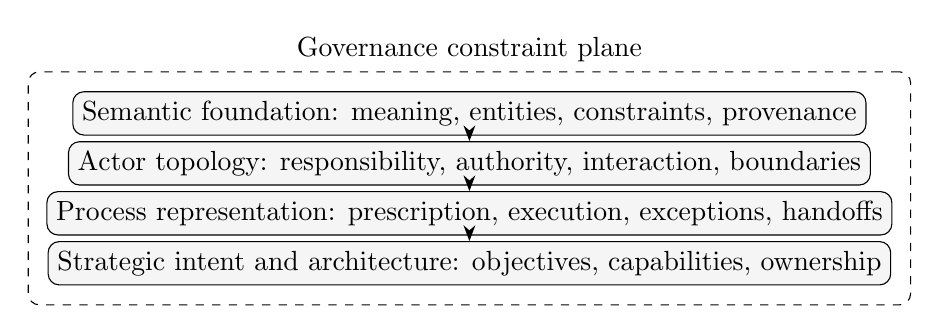
\begin{tikzpicture}[
layer/.style={draw, rounded corners, align=center, minimum width=0.73\textwidth, minimum height=0.55cm, fill=gray!8},
gov/.style={draw, dashed, rounded corners, inner sep=7pt}
]
\node[layer] (semantic) {Semantic foundation: meaning, entities, constraints, provenance};
\node[layer, below=2pt of semantic] (topology) {Actor topology: responsibility, authority, interaction, boundaries};
\node[layer, below=2pt of topology] (process) {Process representation: prescription, execution, exceptions, handoffs};
\node[layer, below=2pt of process] (strategy) {Strategic intent and architecture: objectives, capabilities, ownership};
\node[gov, fit=(semantic)(strategy), label={[align=center]above:Governance constraint plane}] (governance) {};
\draw[-{Stealth[length=2mm]}] (semantic.south) -- (topology.north);
\draw[-{Stealth[length=2mm]}] (topology.south) -- (process.north);
\draw[-{Stealth[length=2mm]}] (process.south) -- (strategy.north);
\end{tikzpicture}
\caption{Reference framework. The four analytical dimensions remain distinct; governance constrains and observes all of them. Cross-layer alignment is examined through relations and evidence, not collapsed into a universal scalar.}
\label{fig:framework}
\end{figure}

\section{The Remaining Alignment Gap}
\subsection{From representational agreement to runtime applicability}
The closest literatures already connect ontologies and workflows, goals and normative frames, actor relationships and trust, and agent proposals with external authorization \parencite{calvanese2026manifesto,jorgensen2026governing}. The unresolved issue examined here is not whether each of these mechanisms ought to exist. It is how an enterprise determines which versions and relationships actually govern a particular action performed by an agent at a particular time. An entity may be correctly resolved while its data-use restrictions remain unknown. A credential may be valid while its delegated scope no longer matches a case assignment. A process transition may be syntactically permitted while the underlying business objective or accountable owner has changed.

This creates a difference between \emph{semantic validity}, \emph{organizational applicability}, \emph{authorization}, and \emph{successful execution}. Semantic validity concerns whether an interpretation is meaningful under a stated model. Applicability asks whether that model and its supporting evidence govern this case, identity, resource, and time. Authorization asks whether the specific action is allowed under applicable constraints and delegated authority. Execution records what occurred, not whether the business outcome was beneficial. A policy engine may evaluate the third question deterministically without independently resolving the first two. Conversely, a neuro-symbolic system can strengthen the first question without becoming the enterprise's authority to approve effects.

Cross-layer alignment therefore describes a relation among representations and their evidential connections, not an additional master ontology or a single policy. The architectural problem includes establishing identity across systems, determining which representation is authoritative for a particular attribute, preserving provenance and version, and distinguishing a stated organizational requirement from an observed but potentially unauthorized practice. Reconciliation should be scoped to a delegated action. A complete computational model of the enterprise is neither assumed nor required.

\subsection{Time, uncertainty, and the speed of change}
Human organizational change often follows committee, process, and release cycles, and a criticism of continuous revalidation is that such context changes slowly. That is only part of the relevant clock. User sessions, workload identities, revocations, resource states, data classifications, service configurations, automated process transitions, and adversarial events can change on software time scales. As agent-created activity becomes more frequent, a system cannot assume that an authorization based on an earlier snapshot remains valid until a person next reviews it. This paper uses a \emph{machine-speed adversarial environment} as a forward-looking threat and design assumption. It does not claim that every attack or organizational attribute is already changing at machine speed.

The consequence is not that every decision must synchronously query every source. Different attributes have different freshness requirements and costs. An organizational owner might be stable for weeks, while revocation or incident quarantine could demand rapid invalidation. Useful designs distinguish evidence age, confidence in its issuer, policy version, expiration, and the operational consequences of relying on stale information. Short-lived grants, event-driven invalidation, local enforcement, and rechecking before consequential effects are plausible mechanisms, but their latency, availability, and safety tradeoffs require evaluation. A check performed before action planning may cease to describe the context at the point of execution; this is a time-of-check-to-time-of-use problem rather than proof that continuous polling will solve every case.

The framework retains three epistemic outcomes: agreement supported by applicable evidence; demonstrated conflict; and unknown or insufficiently trusted evidence. Unknown must not become implicit permission. It may lead to a constrained evidence-gathering step, escalation, or a hold on the consequential action. Determining the correct response is a governance and risk decision, not a choice that an agent should make by inventing a justification.

\subsection{Necessary, supportive, and sufficient conditions}
Cross-layer alignment may support reliable delegation in some settings but is not sufficient for safety, security, legal compliance, or business performance. An aligned set of representations can still be wrong, stale, compromised, or embedded in an insecure runtime. A low-risk, reversible action may be well governed using a small local contract and conventional authorization. Future studies should not infer alignment from success or misalignment from failure without considering model quality, attack, tooling, staffing, and instrumentation as rival explanations.

\section{Integrative Reference Framework}
The paper treats four analytical dimensions and one cross-cutting constraint plane as distinct \emph{architectural concerns}, not five sequential computation stages. Their purpose is to make the relevant enterprise facts discoverable and their relationships inspectable. For a bounded delegated action, the concerns ask what entities and restrictions mean; who bears responsibility and valid authority; what the current process permits; how the action relates to business objectives and architectural dependencies; and what governance requires or prohibits.

\begin{figure}[htbp]
\centering
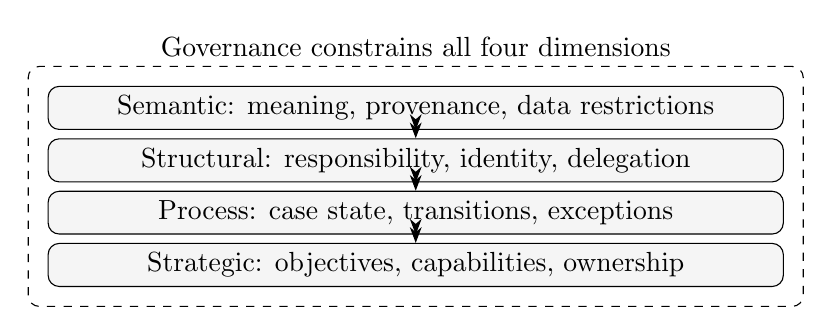
\begin{tikzpicture}[
layer/.style={draw, rounded corners, align=center, minimum width=0.77\textwidth, minimum height=0.53cm, fill=gray!8},
gov/.style={draw, dashed, rounded corners, inner sep=7pt}
]
\node[layer] (semantic) {Semantic: meaning, provenance, data restrictions};
\node[layer, below=3pt of semantic] (topology) {Structural: responsibility, identity, delegation};
\node[layer, below=3pt of topology] (process) {Process: case state, transitions, exceptions};
\node[layer, below=3pt of process] (strategy) {Strategic: objectives, capabilities, ownership};
\node[gov, fit=(semantic)(strategy), label={[align=center]above:Governance constrains all four dimensions}] (governance) {};
\draw[{Stealth[length=2mm]}-{Stealth[length=2mm]}] (semantic.south) -- (topology.north);
\draw[{Stealth[length=2mm]}-{Stealth[length=2mm]}] (topology.south) -- (process.north);
\draw[{Stealth[length=2mm]}-{Stealth[length=2mm]}] (process.south) -- (strategy.north);
\end{tikzpicture}
\caption{Four related organizational representations under cross-cutting governance. Bidirectional connectors indicate dependencies for interpretation and comparison, not a fixed order of execution or a single data pipeline.}
\label{fig:framework}
\end{figure}

\subsection{Context resolution, governed execution, and reconciliation}
The framework is best understood as a recurring interaction among three responsibilities rather than a mandatory new platform. First, authoritative services establish the evidence relevant to the task: entity and data meaning, initiating principal, accountable owner, currently valid delegation, case state, applicable business purpose, and policy constraints. Evidence from an agent's generated narrative remains a claim until verified against its source and applicability. Second, an independent enforcement boundary determines whether a proposed resource access, delegation, tool call, or information transfer is permitted in that scope. Third, outcome and decision evidence is correlated back to organizational context so that investigation, recovery, and organizational change can occur without treating a successful API response as proof of successful enterprise work.

\begin{center}
\small
\fbox{\begin{minipage}{0.89\textwidth}
\centering
\textbf{Delegated task and initiating authority}\\
$\downarrow$\\
\textbf{Resolve applicable, versioned organizational evidence}\\
{\footnotesize Semantics \quad Actor topology \quad Process \quad Strategy \quad Governance}\\
$\downarrow$\\
\textbf{Agent proposes a bounded step or child-agent delegation}\\
$\downarrow$\\
\textbf{Independent context and policy decision at the enforcement boundary}\\
{\footnotesize Permit within scope \quad Deny \quad Resolve missing evidence \quad Escalate}\\
$\downarrow$\\
\textbf{Execute permitted effects, record outcome, and reassess changes}
\end{minipage}}
\end{center}
\noindent\textit{The flow is illustrative. A context-recovery request is not permission to perform the withheld action, and not every low-risk step requires every representation.}

A practical division of responsibility follows. Sources of record establish attributes and their versions; a context resolver associates those attributes with the bounded task; policy and decision services interpret applicable controls; enforcement points mediate actual resource operations; and telemetry links decisions to execution and observed outcomes. An agent may investigate and propose actions, but should not be able to expand its own authority, declare a disputed policy obsolete, or bypass enforcement by selecting another tool. This division is consistent with established Zero Trust and bounded-autonomy work \parencite{nist207a2023,opa2026agent,jorgensen2026governing}. The present paper contributes the enterprise-architecture lens through which their input dependencies and evidence connections can be examined.

\subsection{Multi-level delegated teams}
Dynamic agent teams make organizational structure an execution-time property. A parent agent may create a specialist sub-agent, which may create another child. At each hop, the useful default is \emph{attenuation}: a child receives a narrower scope tied to an explicit subtask, resource set, permitted operation, duration, and downstream delegation limit. A descendant should not obtain authority merely because the parent can ask it to act. Its effective grant should be constrained by the initiating authority, each prior valid delegation, current organizational policy, and task-specific restrictions. Creating a new child should require an independently authorized delegation decision, and the parent should remain attributable without giving every descendant the parent's unrestricted credentials.

Authority can also be withdrawn. Revocation of an upstream grant, reassignment of the responsible role, expiration of a task, or a change in data constraints can invalidate a descendant's access. The architecture therefore needs lineage across the chain and an enforceable revalidation or revocation mechanism. A static RBAC assignment or a prompt instruction alone is not evidence that the lineage remains valid. A hierarchical tree is an illustrative case; actual multi-agent workflows may be graphs with shared services or joint work, requiring explicit treatment of multiple parents and aggregate authority rather than silently taking their union \parencite{tallam2026authorization}.

\subsection{Scalability and operational boundaries}
The long-term enterprise design problem is not a fixed roster of a few agents. Systems may eventually coordinate tens or hundreds of thousands of concurrent agent instances across many processes and resource boundaries. Those counts are planning scenarios, not deployment observations demonstrated by this paper; no architecture has literally infinite capacity. At those scales, centrally resolving every attribute for every intermediate step would create unacceptable latency and failure dependencies. Relevant considerations include identity provisioning, short-lived delegated capabilities, distributed enforcement, local policy evaluation, event-driven invalidation, bounded context retrieval, partitioned telemetry, and proportional retention.

Scaling also changes what must be measured. Throughput and policy-decision latency matter, but so do revocation propagation, stale-decision windows, human escalation load, data exposure, provenance completeness, and business outcomes. A design that increases raw agent concurrency while degrading these properties is not necessarily an improvement. Detailed protocols, consistency guarantees, threat analysis, and performance evaluation belong to a separate technical study; this paper establishes why enterprise context must be represented in that study.


\section{Alignment Dimensions and Operationalization}
\subsection{Semantic alignment}
\textbf{Definition.} Semantic alignment is the extent to which the semantic representations used by humans, agents, processes, systems, and enterprise records are mutually consistent for the bounded work being delegated.

\textbf{Relevant representations.} Ontologies, knowledge graphs, schemas, taxonomies, semantic layers, process vocabularies, entity registries, policy terms, prompts, retrieval sources, and domain definitions are relevant, but they answer different semantic questions.

\textbf{Evidence and candidate observables.} Candidate observables include concept-mapping agreement, unresolved entity references, provenance and version completeness, ontology-to-process links, constraint conflicts, retrieval traceability, exception interpretation, and agreement among domain reviewers. Future measures could compare task-level factual accuracy, domain consistency, constraint adherence, or traceability under bounded interventions.

\textbf{Possible misalignment and consequences.} Misalignment may appear when two representations assign different meanings to a customer, approval, incident severity, or completion state. Consequences may include incorrect routing, invalid decisions, ungrounded explanations, or policy violations.

\textbf{Confounders and boundaries.} A semantic mismatch may be caused by stale data, vocabulary drift, entity-resolution error, retrieval failure, prompt ambiguity, or contested business meaning. The existence of a knowledge graph does not establish semantic alignment, and poor traceability may indicate unknown rather than misaligned meaning.

\textbf{Architectural role and change handling.} A semantic source must be connected to the identity of the business object and the authority of its issuer. A retrieved contract clause, a catalog description, an agent-produced summary, and a current legal amendment cannot be treated as equivalent facts simply because they refer to the same customer. Applicable versions, effective dates, mappings, and provenance matter at the action boundary. Data-centric controls add another dimension: an agent may be permitted to read individual sources while an aggregate, derived summary is subject to different disclosure, retention, or onward-use restrictions. The architecture should preserve enough derivation evidence to evaluate the destination and purpose of a transfer without copying raw sensitive content into general-purpose traces \parencite{w3c2013prov,tallam2026authorization}. Knowledge representation can assist interpretation, but it does not by itself issue enterprise authorization.

\subsection{Structural alignment}
\textbf{Definition.} Structural alignment is the correspondence among responsibility, authority, communication, team or agent boundaries, and system interfaces relevant to the delegated work.

\textbf{Relevant representations.} Prescribed, observed, authorized, and effective actor topologies; role and responsibility records; identity and permission systems; team configurations; service ownership; delegation chains; interaction logs; and software boundaries are relevant.

\textbf{Evidence and candidate observables.} Candidate observables include responsibility gaps or overlaps, authority-permission mismatch, unauthorized delegation paths, topology congruence, cross-boundary interactions, handoff ownership, escalation clarity, and observed versus authorized participation.

\textbf{Possible misalignment and consequences.} Misalignment may occur when an agent acts as if it owns a decision that is assigned to a human, when an authorized identity is substituted at runtime, or when effective escalation bypasses prescribed ownership. Consequences may include accountability ambiguity, unauthorized action, coordination failure, or an incident whose scope is difficult to attribute.

\textbf{Confounders and boundaries.} Organizational charts may lag actual work; event data may omit informal communication; role labels may conceal different authority; and some topology variation is intentional. A difference between prescribed, observed, authorized, and effective topology requires contextual interpretation.

\textbf{Architectural role and change handling.} Actor topology must connect an initiating human or service principal to each participating agent instance, child-agent creation event, capability grant, and resource interaction. The relevant relationship is not just reporting or communication, but who may delegate which subset of operations to whom, for which task, during which interval, and under whose accountability. Agents can be ephemeral while organizational responsibility persists. For multi-level delegation, a child should receive task-specific authority no broader than the valid upstream chain, and a grandchild should be bounded again rather than inherit the parent's full privileges. A policy decision about creating a child is separate from authorization for the child to execute subsequent tools. A revocation or change of accountable owner creates an organizational change event that can affect all live descendants; observed call graphs alone cannot establish the validity of their grants.

\subsection{Process alignment}
\textbf{Definition.} Process alignment is the correspondence among prescribed process context, observed execution, agent actions, decision authority, handoffs, and exception paths.

\textbf{Relevant representations.} BPMN, DEMO, declarative rules, process variants, event logs, tool traces, case records, escalation records, agent plans, and exception-handling artifacts are relevant.

\textbf{Evidence and candidate observables.} Candidate observables include conformance and variant analysis, event completeness, exception coverage, unauthorized transitions, action-to-step traceability, handoff latency, escalation correctness, rework, and human intervention patterns.

\textbf{Possible misalignment and consequences.} Misalignment may appear when a tool call skips a required approval, a process variant is enacted without an allowed exception, or an agent cannot explain how an action relates to the active case state. Consequences may include process failure, hidden work, delayed escalation, duplicate actions, or reduced auditability.

\textbf{Confounders and boundaries.} Event logs are selective; process models can encode idealized work; conformance deviations can be beneficial adaptations; and low event coverage produces unknown evidence rather than automatic nonconformance.

\textbf{Architectural role and change handling.} Process context should distinguish a reusable process definition from the current state of a case instance. An agent may learn that a service credit normally requires approval, but the decision boundary must also determine whether approval for this specific case has already occurred, whether that approval remains valid, and whether the action has been executed already. Tool-success events, process transitions, approval records, and compensating transactions need stable correlation identifiers. A lengthy delegated workflow may span multiple context versions; an approval recorded at planning time may not authorize execution after an incident hold or case reassignment. An exception path should be explicit and reviewable rather than guessed from previous successful executions. This does not imply that every workflow must use BPMN or a central process engine.

\subsection{Strategic alignment}
\textbf{Definition.} Strategic alignment is the correspondence among delegated behavior, enterprise objectives, capabilities, architecture, service ownership, and risk posture.

\textbf{Relevant representations.} Objectives, capability maps, value streams, architecture viewpoints, service catalogs, ownership records, risk registers, investment decisions, policy priorities, and agent task specifications are relevant.

\textbf{Evidence and candidate observables.} Candidate observables include objective-to-action traceability, capability and owner links, architecture dependency consistency, policy-objective conflict, risk-tolerance exceptions, change history, and decisions that explain why autonomy was granted.

\textbf{Possible misalignment and consequences.} Misalignment may occur when an agent optimizes a local service metric that conflicts with a stated enterprise objective, or when architecture assigns ownership differently from the operating model. Consequences may include local optimization, duplicated capability, unowned risk, resource conflict, or strategic drift.

\textbf{Confounders and boundaries.} Strategic intent can be contested, tacit, or changing. Traceability does not establish agreement, effectiveness, or ethical acceptability. The framework therefore treats strategic alignment as contextual and reviewable rather than as a static label.

\textbf{Architectural role and change handling.} Business purpose is part of a delegation's legitimacy, not merely a reporting label. A locally efficient agent can satisfy a narrow task metric while exceeding a risk budget, harming a long-term customer relationship, or contradicting an enterprise decision to retain human authority over exceptions. An architectural context view therefore connects the delegated outcome to the initiating business objective, relevant capability, service owner, target system, and recorded risk posture. It also needs to preserve legitimate disagreement: two units may have competing priorities, and a policy engine cannot invent a universal ordering among them. Where objectives conflict materially, escalation or an explicitly governed trade-off is more defensible than treating a model's inferred preference as enterprise intent.

\subsection{Governance as a constraint plane}
\textbf{Definition.} Governance is the cross-cutting set of constraints and oversight mechanisms that defines permissible identity, permission, prohibition, obligation, delegation, approval, separation of duties, monitoring, attribution, audit, revocation, interruptibility, and autonomy boundaries.

\textbf{Relevant representations.} Identity records, authorization policies, policy versions, approval records, separation-of-duties rules, delegation chains, monitoring and audit logs, revocation events, interruption controls, incident records, and human oversight procedures are relevant.

\textbf{Evidence and candidate observables.} Candidate observables include identity-to-action traceability, policy decision records, approval and escalation evidence, permission drift, separation-of-duties conflicts, monitoring coverage, attribution completeness, revocation latency, interruption success, and boundary violations. No numeric governance coverage is assumed.

\textbf{Possible misalignment and consequences.} Misalignment may occur when a capable agent is permitted to act outside a stated boundary, when a prohibition is not enforced at the tool boundary, when a delegation chain lacks an accountable principal, or when monitoring cannot distinguish agent and human action. Consequences may include unauthorized action, non-repudiation gaps, unreviewable decisions, or inability to stop a harmful action.

\textbf{Confounders and boundaries.} Policy language may be ambiguous or stale; identity may be shared; logs may be incomplete; monitoring may exist without meaningful review; and governance controls can add friction that changes behavior. Governance evidence should therefore be evaluated for scope, freshness, enforcement point, and attribution quality.

\textbf{Architectural role and change handling.} Governance distinguishes three responsibilities: formulating policy and accountable decisions; evaluating a particular proposed action against policy and verified attributes; and enforcing the resulting disposition at the resource or tool boundary. The last responsibility must not rely solely on an agent voluntarily following instructions. A permit should be scoped to a particular subject, action, resource, purpose, and applicable conditions; a prior permit is not a blanket approval for descendants or future effects. Denial, missing evidence, explicit exceptions, and human escalation should remain distinguishable for operations and audit, even if a particular PDP emits a simpler decision vocabulary. Distributed enforcement must address local policy versions, revocation events, bounded decision caching, and fail-closed behavior for consequential actions when critical attributes are unavailable. Zero Trust principles support those boundaries, but do not supply the correct enterprise-specific policy or ensure beneficial results \parencite{nist207a2023,opa2026agent}.

The five concerns describe different kinds of organizational evidence; they are not five independent scores. In practice the same business activity crosses several concerns. An architectural review should trace at least one bounded task from initiating business purpose through identity and context resolution, action authorization, execution, and outcome evidence. This reveals whether a proposed agent integration is merely technically connected or also supports accountable organizational action.

\section{Cross-Layer Mismatch and Failure Modes}
The operational center of the framework is not ''what is the score?'' but ''where do representations disagree, and what evidence supports that conclusion?'' A cross-layer mismatch is a context-specific divergence among representations relevant to the same bounded action. A divergence can be intentional, temporary, adaptive, benign, or harmful. It becomes an alignment concern when the task, authority, risk, and evidence indicate that the divergence can create an unacceptable responsibility, process, semantic, strategic, or governance problem. If evidence is insufficient, the correct classification is unknown rather than misaligned.

\subsection{Illustrative case: successful tool execution, incorrect enterprise action}
Consider a customer-support agent assigned to resolve a billing dispute. Its CRM lookup identifies the correct customer, and its credit-issuance API returns success. An evaluation that examines only tool syntax and task completion would record a successful result. Yet the customer contract was amended that morning, the recorded process approval threshold refers to the prior contract, the account moved to a different team, and the agent's service identity retains permissions granted under the old operating model. Each source may be locally accurate for its own timestamp. Their combination is not necessarily applicable to this action.

A cross-layer investigation should establish which contract terms applied at the time of the credit; how the service case and accountable owner were resolved; which approval or exception was required for that case; whether the effective identity and delegation were authorized; and whether the resulting credit complied with the current risk and customer objectives. The agent could be permitted to retrieve authoritative evidence while the credit action remains held for clarification. If a valid policy prohibits issuance, the resource boundary should deny the call even when the agent's plan is coherent. The resulting record should connect the selected evidence and policy version to the observed API effect so that a reviewer can reconstruct the business decision. The value is not an obvious reminder to check permissions; it is the ability to detect that a \emph{successful} local execution was based on a mixture of organizational states that should not have been composed.

\subsection{Illustrative case: dynamic delegation and derived-data disclosure}
Consider an orchestrator that creates a temporary research agent to inspect a customer's incident, and that agent creates two specialists to examine separate financial and security records. Each specialist receives only the source-specific access and operations needed for its assigned subtask, not the full authority of its parent. A summarizing agent later combines their outputs. During execution, an incident hold revokes part of the initiating task's authority. A local policy cache on one tool gateway has not yet seen the change.

Several decisions must remain distinct. The sub-agent creation decision must validate task scope and upstream delegation. Each retrieval must use the child's actual identity and applicable purpose. The combined report may carry a disclosure restriction that neither source alone made obvious to a reader of the intermediate outputs. Before release, an enforcement boundary must apply destination and data-derivation constraints to the resulting artifact. Revocation should prevent subsequent consequential accesses or transfers within the system's stated freshness and availability assumptions. If lineage or classification is incomplete, an unknown evidentiary state should cause further permitted inquiry or human escalation, not invented permission.

The hypothetical failure is not simply an unauthorized tool call. It is a mismatch among temporal authority, hierarchical topology, information provenance, and downstream purpose. Detecting or preventing it may incur authorization latency, data-labeling work, false holds, and extra human review. These costs must appear beside any security benefit. Neither case is empirical evidence; both specify situations in which the cross-layer framing can be compared with simpler local controls.

\begingroup
\scriptsize
\setlength{\tabcolsep}{2pt}
\renewcommand{\arraystretch}{1.15}
\begin{longtable}{P{0.15\textwidth} P{0.18\textwidth} P{0.27\textwidth} P{0.30\textwidth}}
\caption{Mismatch patterns for empirical observation and case analysis.}\label{tab:mismatches}\\
\toprule
\textbf{Mismatch} & \textbf{Compared representations} & \textbf{Example disagreement} & \textbf{Evidence, consequence, or caveat} \\
\midrule
\endfirsthead
\toprule
\textbf{Mismatch} & \textbf{Compared representations} & \textbf{Example disagreement} & \textbf{Evidence, consequence, or caveat} \\
\midrule
\endhead
Semantic--process & Semantic foundation and process representation & A ''resolved'' case has different meanings in the domain vocabulary and process state model. & Compare mappings, definitions, provenance, and state transitions. Consequences may include wrong routing or invalid completion. A vocabulary difference may be a deliberate local variant; stale definitions create unknown evidence until checked. \\
Structural--governance & Actor topology and governance plane & A role is responsible for a decision, but the identity and permission system grants the action to another principal. & Compare role, responsibility, identity, permission, and delegation records. Consequences may include accountability gaps or unauthorized action. Shared-service design can make the difference intentional. \\
Process--topology & Process representation and actor topology & The prescribed handoff assigns a human reviewer, while observed execution routes the decision through an agent with no recorded delegated authority. & Use event, identity, handoff, and authorization traces. Consequences may include hidden responsibility transfer. Missing telemetry establishes an observability limitation, not necessarily a breach. \\
Strategic--process & Strategic intent and process representation & A local optimization removes an escalation step that enterprise risk policy treats as mandatory. & Compare objective traceability, policy priorities, process variants, and change records. Consequences may include strategic drift or risk exposure. Objectives can conflict or change over time. \\
Semantic--governance & Semantic foundation and governance plane & ''Sensitive customer data'' is defined differently in a data ontology and an access policy. & Inspect term mappings, policy versions, data classifications, and policy decisions. Consequences may include improper access. A definition conflict may be unresolved rather than empirically established. \\
Observed--prescribed & Observed effective work and prescribed process or topology & Informal escalation is routinely used but does not appear in the process model or ownership record. & Compare event and communication evidence with models and interview accounts. The difference may be safe adaptation, process debt, or tacit knowledge; classification needs context. \\
Authorized--observed topology & Authorized topology and observed topology & A service account executes cross-boundary actions that are not represented in the authorized delegation path. & Compare runtime identities, delegation chains, interaction logs, and tool traces. Consequences may include unauthorized edges or enlarged blast radius. Identity correlation errors can make the status unknown. \\
Process--governance & Process representation and governance plane & A process step permits an action that a current prohibition or approval rule disallows. & Compare process versions, policy decisions, approval records, and enforcement points. Consequences may include blocked work or prohibited execution. A stale process repository can explain the discrepancy. \\
Semantic--structural & Semantic foundation and actor topology & The concept of ''case owner'' is mapped to a service account rather than the accountable team role. & Compare entity and role mappings, ownership records, and task assignments. Consequences may include ownership ambiguity. Terminology variation alone is not misalignment. \\
Architecture--organizational ownership & Enterprise architecture and organizational ownership & A system dependency is owned by a platform team, while the operating model assigns the corresponding capability to a product team. & Compare architecture repositories, service catalogs, capability maps, and operating-model records. Consequences may include unowned changes or incident handoff failure. Transitional reorganizations can be intentional. \\
Strategic intent--granted autonomy & Strategic intent and granted autonomy & An agent receives broad write authority for a task whose stated risk posture requires human approval and reversibility. & Compare autonomy decisions, permissions, risk appetite, approval gates, and revocation tests. Consequences may include inappropriate exposure. Technical capability is not evidence of strategic authorization. \\
\bottomrule
\end{longtable}
\endgroup

The table is a diagnostic catalog, not a prevalence claim. The same difference can receive different classifications in different contexts. A defensible analysis records task scope, representation versions, evidence provenance, affected boundaries, and unresolved alternatives.

\section{Benefit and Research Propositions}
The propositions below are intentionally bounded and evidence-labeled. They are prompts for empirical work, not claims that the synthesis has validated.

\begingroup\scriptsize
\begin{longtable}{p{0.08\textwidth} p{0.38\textwidth} p{0.18\textwidth} p{0.27\textwidth}}
\caption{Propositions and evidence boundaries.}\label{tab:propositions}\\
\toprule
ID & Proposition & Evidence category & Boundary condition \\
\midrule
\endfirsthead
\toprule
ID & Proposition & Evidence category & Boundary condition \\
\midrule
\endhead
P1 & Shared semantic representations can improve factual accuracy, domain consistency, constraint adherence, or traceability for bounded agent tasks relative to otherwise comparable ungrounded conditions. & Strong adjacent; emerging direct & Effects depend on coverage, freshness, retrieval, entity resolution, and task design; semantic grounding does not guarantee truth. \\
P2 & Better-specified actor topology and bounded authority can improve responsibility clarity and expose or constrain interactions inconsistent with assigned authority. & Emerging direct; strong adjacent & Incident blast radius is a future outcome to test, not an established consequence. Topology variation may be intentional or poorly observed. \\
P3 & Explicit process representations and event evidence can expose exception, conformance, handoff, and attribution failures that are difficult to see from aggregate task success. & Strong adjacent; emerging direct & Event data omit tacit work and uninstrumented channels; inspectability does not automatically prevent failure. \\
P4 & For some consequential delegated tasks, connecting semantic, structural, process, strategic, and governance evidence at the runtime boundary may improve decisions beyond isolated local controls. & Conceptual / speculative & Compare against authorization overhead, false holds, and simpler controls that may perform equally well. \\
P5 & Explicitly representing uncertainty and separating alignment, misalignment, and unknown evidence can improve the quality of autonomy, escalation, and review decisions. & Conceptual / emerging & The representation can add bureaucracy or false confidence; studies must measure decision quality and negative cases. \\
P6 & Context freshness and revocation propagation become more consequential as automated execution and adversarial changes outpace periodic human review. & Strong adjacent; conceptual transfer & Not all attributes change rapidly. Compare stale-permit windows, availability, and latency under specified workloads. \\
P7 & Multi-level, task-scoped delegation can constrain descendant authority and exposure relative to unconstrained credential inheritance. & Strong adjacent; emerging direct & Derived grants need independent enforcement, including transfers and changing workflow branches; privilege aggregation remains a challenge. \\
\bottomrule
\end{longtable}
\endgroup

P4 is the central integration proposition, and it remains the least empirically established. An empirical result showing no interaction among dimensions would still be important: it would constrain the value of a cross-layer framework and reveal when local controls are sufficient. Conversely, a positive interaction would need to be separated from confounding improvements in instrumentation, staffing, training, prompting, or review.

\subsection{Enterprise value and its operating costs}
The potential enterprise benefit is not another governance dashboard. If context and enforcement are reusable across applications and agent frameworks, an organization may be able to delegate a broader range of bounded actions without embedding separate authorization, process interpretation, and review systems within each agent. Better evidence might also reduce investigation effort and expose costly local optimization. These are mechanisms to investigate, not measured returns on investment.

\begin{table}[htbp]
\centering\small
\begin{tabular}{P{0.28\textwidth} P{0.32\textwidth} P{0.28\textwidth}}
\toprule
Potential outcome & Evidence worth comparing & Countervailing cost \\
\midrule
Greater appropriate autonomy & Completed cases without inappropriate action or unnecessary escalation & Decision latency, failed legitimate tasks \\
More accountable execution & Reconstruction of actor, applicable context, approval, and resulting effect & Telemetry volume, privacy and retention burden \\
Faster recovery after change & Revocation propagation, stale decisions, recovery effort & Cache invalidation, service dependency, availability \\
Less duplicated integration & Reusable context contracts and policy decisions across workflows & Mapping, ownership, and governance maintenance \\
\bottomrule
\end{tabular}
\caption{Candidate enterprise benefits and costs; none is an established effect of this framework.}
\end{table}

The design should preserve a low-cost path for narrow, reversible operations where local controls are adequate. Adding cross-layer lookups to every inference step would impose complexity without necessarily adding security or economic value.

\section{Candidate Observables and Optional DTO Substrate}
Candidate observables are listed to make the synthesis empirically approachable. They are not validated metrics, confidence estimates, governance coverage scores, or a predetermined composite. Researchers should choose measures that fit a bounded task, preregister the comparison, record representation versions, and report missing evidence as unknown where appropriate.

\begingroup\scriptsize
\begin{longtable}{p{0.15\textwidth} p{0.22\textwidth} p{0.25\textwidth} p{0.28\textwidth}}
\caption{Candidate observables without assuming a universal scoring function.}\label{tab:observables}\\
\toprule
Dimension & Objects examined & Candidate observable evidence & Limits and confounders \\
\midrule
\endfirsthead
\toprule
Dimension & Objects examined & Candidate observable evidence & Limits and confounders \\
\midrule
\endhead
Semantic & Concepts, entities, mappings, constraints, provenance, retrieval sources & Mapping review, entity-resolution errors, policy-term conflicts, traceability, bounded task accuracy, constraint adherence & Domain drift, stale sources, ambiguous labels, and retrieval selection can alter results. \\
Structural & Roles, responsibility, authority, delegation, team and system boundaries, interactions & Ownership records, authorization traces, delegation chains, handoff ownership, observed versus authorized topology & Shared identities, missing communication data, reorganizations, and intentional adaptation complicate interpretation. \\
Process & Models, cases, events, variants, exceptions, handoffs, agent actions & Conformance, event completeness, exception coverage, action-to-step traceability, escalation and handoff records & Event logs are selective; model quality and instrumentation can explain apparent effects. \\
Strategic & Objectives, capabilities, architecture, service ownership, risk appetite & Objective-to-action traceability, owner links, architecture dependencies, policy-objective conflicts, autonomy decisions & Intent can be tacit, contested, changing, or decoupled from formal artifacts. \\
Governance & Identity, permission, prohibition, obligation, approval, monitoring, audit, revocation, interruption & Policy decision records, identity-to-action links, approval evidence, separation-of-duties checks, revocation and interruption tests & A recorded control may be stale, unenforced, or unreviewed; no numeric coverage is assumed. \\
\bottomrule
\end{longtable}
\endgroup

\subsection{An action-centered evidence contract}
Telemetry becomes useful for cross-layer analysis only when the same bounded activity can be traced through its organizational context and resulting effect. An implementation need not persist every retrieved document or model prompt. It should be able to preserve a protected, correlatable evidence record sufficient to reconstruct which facts, identities, policies, and resource states were considered. W3C PROV-O supplies a conceptual vocabulary for derivation and responsibility; emerging OpenTelemetry agent and workflow spans describe runtime operations but should not be treated as a complete governance schema \parencite{w3c2013prov,otel2026agent}.

\begin{longtable}{P{0.23\textwidth} P{0.38\textwidth} P{0.27\textwidth}}
\caption{Candidate evidence fields for bounded delegated action; an illustrative contract, not a proposed universal schema.}\label{tab:action-evidence}\\
\toprule
Evidence category & Minimum question the record should support & Collection and interpretation boundary \\
\midrule
\endfirsthead
\toprule
Evidence category & Minimum question the record should support & Collection and interpretation boundary \\
\midrule
\endhead
Task and purpose & Which case and objective initiated the request; what effect was sought? & Limit business-context exposure and keep identifying data protected. \\
Actor and chain & Which human, service, agent instance, and delegation ancestry were involved? & Avoid shared identities; validate source of identity assertions. \\
Action target & Which resource, operation, recipient, and intended result were in scope? & A proposed operation may differ from the executed one. \\
Context and versions & Which organizational facts, process state, classifications, and policy versions were applicable? & Reference authoritative snapshots; record effective time and freshness. \\
Decision and obligation & What PDP disposition, reasons, obligations, expiration, and exception path applied? & Policy evaluation is not proof of correct business outcome. \\
Execution and transfer & Did the PEP allow or block an effect, and to whom was data transferred? & Enforcement and downstream release require separate coverage. \\
Outcome and change & What effect was observed, what changed subsequently, and was revocation applied? & Correlation alone does not establish cause or absence of leakage. \\
\bottomrule
\end{longtable}

Evidence quality is a property of the resulting trace, not a multiplier on alignment. If an identity assertion is unverified, a policy version cannot be determined, a child-agent edge is missing, or a source classification is ambiguous, the correct result is an explicit evidence gap. Sensitive raw content should not be copied into general-purpose telemetry merely to obtain trace completeness. Data minimization, tamper evidence, access control, retention, and compartmented investigation are first-class design constraints. A partial distributed evidence graph can be more defensible than a supposedly complete centralized twin.

\subsection{Decision freshness and feedback}
A context change may arrive as a new process event, revised policy, identity revocation, incident signal, amended data label, or updated service ownership. The system needs a stated way to invalidate affected decisions or re-evaluate a later action using current authoritative inputs. That may involve event subscriptions, locally checked short-lived grants, or synchronous PDP calls for high-impact effects. Eventual consistency creates a period in which two enforcement points can see different context; the residual exposure needs to be measured and accepted by the relevant governance authority rather than concealed by a generic assertion of continuous authorization.

This is also a business feedback loop. A legitimate request that is repeatedly blocked due to stale mappings, missing approvals, or excessive revalidation reveals design debt and economic costs. Operational review should distinguish a prevented unauthorized operation, a false denial, an unnecessary escalation, and a successful outcome. These distinctions allow the value of cross-layer context to be tested against simpler controls without relying on a universal numeric alignment index.

\subsection{DTO as an optional evidence substrate}
A DTO-like substrate can link partial, versioned, observable representations of an organization. One implementation might connect semantic entities and provenance; actor identities, roles, responsibilities, authority, interfaces, and boundaries; prescribed process models and observed event traces; objectives, capabilities, architecture dependencies, owners, and risk relations; and agent traces that connect actions to tools, process steps, data sources, approvals, policy decisions, and outcomes.

The substrate need not perfectly model the enterprise and is not necessary for the framework. Its value would be in preserving links, versions, scope, provenance, uncertainty, and the distinction between explicit, observed, inferable, and tacit knowledge. It could support case comparison, drift detection, audit queries, and counterfactual study. It cannot infer omitted tacit knowledge automatically, make an organizational objective uncontested, or convert correlation into causal evidence. Its usefulness depends on identity resolution, instrumentation, access control, privacy, and model governance.

The repository retains a small exploratory mismatch catalog to make the categories concrete. That code is scaffolding for discussion and future data work; it is not a paper contribution, validator, safety calculator, or source of research evidence.

\section{Empirical Research Agenda}
\subsection{Construct usefulness}
Study whether practitioners, researchers, and domain reviewers find the four-dimension-plus-governance vocabulary useful for diagnosing bounded delegated work. Compare the cross-layer framing with local semantic, process, architecture, teaming, and governance reviews. Record cases where the framework adds no information or creates unhelpful duplication.

\subsection{Inter-rater reliability}
Give independent reviewers the same scoped artifacts and ask them to classify alignment, misalignment, and unknown across the mismatch catalog. Measure disagreement, adjudication effort, sensitivity to representation version, and the effect of domain expertise. Reliability work should be reported as evidence about the classification protocol, not as proof that the underlying organization is aligned.

\subsection{Observable indicators and outcome association}
Identify observable indicators for each dimension using bounded, versioned data: ontology and policy mappings, identity and delegation records, event traces, handoff and escalation records, architecture ownership, and human outcome measures. Test association with task correctness, exception resolution, accountability clarity, calibrated reliance, unauthorized action, auditability, rollback time, or incident scope. Avoid assuming in advance that these indicators should combine into one equation.

\subsection{Interaction and comparative designs}
Use factorial, quasi-experimental, or longitudinal designs to vary semantic, structural, process, strategic, and governance conditions independently where feasible. Compare isolated interventions with cross-layer interventions. A null interaction is a meaningful result. Positive association should be tested against confounding by instrumentation, training, staffing, prompting, permissions, and review.

\subsection{Boundary conditions and negative cases}
Sample reversible low-risk tasks, regulated high-impact work, exception-rich cases, cross-functional handoffs, and long-horizon delegated actions. Examine how tacit knowledge, changing objectives, adversarial input, tool failures, identity substitution, stale policies, and incomplete event data alter classification and outcomes. Publish negative cases in which explicit modeling increases bureaucracy, a topology intervention harms flow, or a semantic layer creates false confidence.

\subsection{DTO and replication}
Begin with bounded processes and de-identified, versioned evidence. Share schemas, representation mappings, case-selection rules, classification protocols, and analysis code where lawful. Replicate across claims, customer support, compliance triage, and incident response without treating those use cases as interchangeable. A DTO implementation should follow evidence and privacy requirements rather than be assumed as a prerequisite.

\subsection{Machine-speed change, delegated depth, and scale}
Future evaluation should explicitly vary the rate of context changes relative to agent action rates, including bursts of revocation, reassignment, and adversarial policy or identity events. Compare stale-permit windows, denied legitimate work, context-recovery latency, policy-decision latency, revocation propagation, and eventual convergence. Distinguish low-risk reads from costly external effects. Compare one-level and multi-level delegation, branching and shared-subagent topologies, partial loss of parent authority, and aggregation of separately permitted data.

Claims of large-scale applicability require stated workloads and measured resource consumption. A useful experimental sequence might progress from a small controlled test to thousands and then tens or hundreds of thousands of simulated concurrent agent instances, if feasible. Report agents, tasks, policy decisions, resources, and events separately; agent count alone is not throughput. Evaluate central versus distributed policy decision points, caching and invalidation policies, partition recovery, event sampling, tenant separation, and degraded connectivity. This paper supplies the questions and design pressures, not empirical results or an unbounded scalability guarantee.

\section{Threats to Validity}
Construct validity is threatened by treating labels such as agent, role, process, or alignment as interchangeable across literatures. The definitions in this paper reduce that risk but do not establish community-wide agreement. Content validity is threatened by omitting relevant work from a focused search. The method records search terms, source classes, inclusion rules, chaining, and gaps, but it is not exhaustive.

Internal validity is threatened by confounding: an intervention that appears to improve alignment may also improve instrumentation, training, prompting, permissions, staffing, or review. An apparent benefit may therefore be attributable to process discipline or additional oversight rather than cross-layer interaction. External validity is threatened by variation in regulation, process maturity, data quality, organization size, agent architecture, and tacit practice.

Evidence classification is uncertain for rapidly moving 2025--2026 work. Practitioner sources, standards, workshop papers, proceedings abstracts, and preprints are retained with explicit labels; they should not be silently promoted to peer-reviewed empirical evidence. The proposed mismatch classifications also depend on scope, version, provenance, and reviewer interpretation. Finally, the exploratory code is a reproducibility aid for the taxonomy, not a validating model or source of empirical evidence.

\section{Limitations and Boundary Conditions}
\subsection{Higher applicability}
The framework is more applicable when work is cross-functional, regulated, high-impact, long-horizon, exception-rich, delegated across software boundaries, or difficult to reverse. It is also more useful when multiple teams use inconsistent terms, responsibility and authority are separated, or the organization needs an auditable account of why an agent acted.

\subsection{Lower applicability}
The framework is less necessary as a broad organizational representation for narrow, low-risk, reversible, well-instrumented actions with stable semantics, local authority, and little exception variation. A simple agent that classifies a bounded input or retrieves a document may need only a small semantic and permission contract.

The synthesis is limited by its purposive literature scope, qualitative mappings, manually audited bibliography, and absence of primary field data. It does not offer a production architecture, compliance certification, causal effect estimate, universal autonomy threshold, or claim that all organizational knowledge can be represented. Machine-speed adversarial change and very large agent populations are forward-looking scenarios, not measured deployment prevalence. Proposed evidence contracts, revocation behavior, and hierarchical delegation illustrate architectural questions, not verified protocol properties. The paper does not treat missing explicit representation as automatic misalignment or resolve how tacit knowledge should be elicited without surveillance, excessive bureaucracy, or false completeness.

\section{Conclusion}
Agentic BPM, Human--AI Teaming, semantic BPM, process mining, enterprise architecture, governance, and DTO research already provide substantial pieces of the human-agent enterprise problem. This paper brings those pieces into a cross-layer framing in which alignment means evidence-supported correspondence among meaning, actors, process, intent, and governance. The goal is to provide a practical basis for conceptual comparison and empirical study.

The framework's practical center is the relationship between applicable organizational evidence and delegated action. Prescribed, observed, authorized, and effective representations may agree, conflict, or remain unknown; governance constrains the use of all four dimensions. Machine-speed context changes, multi-hop ephemeral delegation, and data derivation make that relation operationally important, while distributed evidence and independent enforcement create additional cost and consistency questions. The proposed scenarios and evidence contract illustrate how enterprise architects can study that relation without assuming a complete digital twin or an always-current graph. Whether such connections improve business outcomes, security, or appropriate autonomy beyond simpler local controls remains a question for comparative evaluation. The repository's experimental catalog illustrates the vocabulary; it validates neither a score nor a security protocol.

\begin{thebibliography}{99}
\bibitem{gruber1993translation} Gruber, T. R. (1993). A translation approach to portable ontology specifications. \emph{Knowledge Acquisition}, 5(2), 199--220. \url{https://doi.org/10.1006/knac.1993.1008}.
\bibitem{guarino1998formal} Guarino, N. (1998). Formal ontology and information systems. In N. Guarino (Ed.), \emph{Proceedings of FOIS'98}, 3--15.
\bibitem{dietz2006enterprise} Dietz, J. L. G. (2006). \emph{Enterprise Ontology: Theory and Methodology}. Springer.
\bibitem{w3cowl2004} W3C. (2004). \emph{OWL Web Ontology Language Semantics and Abstract Syntax}. \url{https://www.w3.org/TR/owl-semantics/}.
\bibitem{w3cskos2009} W3C. (2009). \emph{SKOS Simple Knowledge Organization System Reference}. \url{https://www.w3.org/TR/skos-reference/}.
\bibitem{hepp2005semantic} Hepp, M., Leymann, F., Domingue, J., Wahler, A., \& Fensel, D. (2005). Semantic business process management: A vision towards using semantic Web services for business process management. In \emph{IEEE International Conference on E-Business Engineering}, 535--540.
\bibitem{annane2019bbo} Annane, A., Ravat, F., Teste, O., \& Ternisien, A. (2019). BBO: An ontology for representing business process models. In \emph{Proceedings of the 11th International Joint Conference on Knowledge Discovery, Knowledge Engineering and Knowledge Management}.
\bibitem{omg2014bpmn} Object Management Group. (2013). \emph{Business Process Model and Notation (BPMN), Version 2.0.2}. \url{https://www.omg.org/spec/BPMN/2.0.2/PDF/}.
\bibitem{aalst2016process} van der Aalst, W. M. P. (2016). \emph{Process Mining: Data Science in Action} (2nd ed.). Springer.
\bibitem{skelton2019team} Skelton, M., \& Pais, M. (2019). \emph{Team Topologies: Organizing Business and Technology Teams for Fast Flow}. IT Revolution Press.
\bibitem{wooldridge1995intelligent} Wooldridge, M., \& Jennings, N. R. (1995). Intelligent agents: Theory and practice. \emph{The Knowledge Engineering Review}, 10(2), 115--152. \url{https://doi.org/10.1017/S0269888900008122}.
\bibitem{dorri2018multiagent} Dorri, A., Kanhere, S. S., \& Jurdak, R. (2018). Multi-agent systems: A survey. \emph{IEEE Access}, 6, 28573--28593. \url{https://doi.org/10.1109/ACCESS.2018.2831228}.
\bibitem{conway1968committees} Conway, M. E. (1968). How do committees invent? \emph{Datamation}, 14(4), 28--31.
\bibitem{macCormack2012exploring} MacCormack, A., Baldwin, C., \& Rusnak, J. (2012). Exploring the duality between product and organizational architectures: A test of the mirroring hypothesis. \emph{Research Policy}, 41(8), 1309--1324. \url{https://doi.org/10.1016/j.respol.2012.04.011}.
\bibitem{zachman1987framework} Zachman, J. A. (1987). A framework for information systems architecture. \emph{IBM Systems Journal}, 26(3), 276--292.
\bibitem{togaf2022standard} The Open Group. (2022). \emph{The TOGAF Standard, 10th Edition}. \url{https://pubs.opengroup.org/togaf-standard/}.
\bibitem{archimate2022standard} The Open Group. (2022). \emph{ArchiMate Specification, Version 3.2}. \url{https://pubs.opengroup.org/archimate-spec/}.
\bibitem{lewis2020retrieval} Lewis, P., Perez, E., Piktus, A., Petroni, F., Karpukhin, V., Goyal, N., K{\"u}ttler, H., Lewis, M., Yih, W.-t., Rockt{\"a}schel, T., Riedel, S., \& Kiela, D. (2020). Retrieval-augmented generation for knowledge-intensive NLP tasks. In \emph{Advances in Neural Information Processing Systems}, 33. \url{https://proceedings.neurips.cc/paper/2020/file/6b493230205f780e1bc26945df7481e5-Paper.pdf}.
\bibitem{pan2024unifying} Pan, S., Luo, L., Wang, Y., Chen, C., Wang, J., \& Wu, X. (2024). Unifying large language models and knowledge graphs: A roadmap. \emph{IEEE Transactions on Knowledge and Data Engineering}, 36(7), 3580--3599. \url{https://doi.org/10.1109/TKDE.2024.3352100}.
\bibitem{sarker2021neuro} Sarker, I. H. (2022). Neuro-symbolic AI: The state of the art. \emph{Applied Intelligence}, 52, 6859--6885. \url{https://doi.org/10.1007/s10489-021-03036-1}.
\bibitem{polanyi1966tacit} Polanyi, M. (1966). \emph{The Tacit Dimension}. University of Chicago Press.
\bibitem{nonaka1995knowledge} Nonaka, I., \& Takeuchi, H. (1995). \emph{The Knowledge-Creating Company}. Oxford University Press.
\bibitem{dumas2023abpms} Dumas, M., Fournier, F., Limonad, L., Marrella, A., Montali, M., Rehse, J.-R., Rozumnyi, S., Vu, M. N., \& Weber, B. (2023). AI-augmented business process management systems: A research manifesto. \emph{ACM Transactions on Management Information Systems}, 14(1), Article 11. \url{https://doi.org/10.1145/3576047}.
\bibitem{tour2023agentminer} Tour, A., Polyvyanyy, A., Kalenkova, A., \& Senderovich, A. (2023). Agent Miner: An algorithm for discovering agent systems from event data. In \emph{Business Process Management}, LNCS 14159, 284--302. \url{https://doi.org/10.1007/978-3-031-41620-0_17}.
\bibitem{calvanese2025normative} Calvanese, D., De Giacomo, G., Kampik, T., Lesperance, Y., Marrella, A., \& Matta, A. (2025). Autonomy in business process execution: Why we need first-class abstractions for goals and normative frames. In \emph{Proceedings of the International Workshop on Process Management in the AI Era}.
\bibitem{vu2025agentic} Vu, H., Klievtsova, N., Leopold, H., Rinderle-Ma, S., \& Kampik, T. (2025). Agentic business process management: The past 30 years and practitioners' future perspectives. arXiv:2504.03693. \url{https://arxiv.org/abs/2504.03693}.
\bibitem{dumas2026abpms} Dumas, M., Milani, F., \& Chapela-Campa, D. (2026). Agentic business process management systems. In \emph{Business Process Management Workshops}, LNBIP 569, 3--14. \url{https://doi.org/10.1007/978-3-032-13426-4_1}.
\bibitem{calvanese2026manifesto} Calvanese, D., Casciani, A., De Giacomo, G., Dumas, M., Fournier, F., Kampik, T., La Malfa, E., Limonad, L., Marrella, A., Metzger, A., Montali, M., Amyot, D., Fettke, P., Polyvyanyy, A., Rinderle-Ma, S., Sardiña, S., Tax, N., \& Weber, B. (2026). Agentic business process management: A research manifesto. \emph{Information Systems}, 140, 102738. \url{https://doi.org/10.1016/j.is.2026.102738}.
\bibitem{degiacomo2026formal} De Giacomo, G., Kampik, T., Kirchdorfer, M., Montali, M., \& Weinhuber, M. (2026). Formal foundations of agentic business process management. arXiv:2604.17347. \url{https://arxiv.org/abs/2604.17347}.
\bibitem{bala2026agents} Bala, S., Fournier, F., Limonad, L., \& Metzger, A. (2026). Using process mining to generate AI agents from software engineering process records. arXiv:2607.04948. \url{https://arxiv.org/abs/2607.04948}.
\bibitem{orgmining2026} Shen, Q., Polyvyanyy, A., Lipovetzky, N., \& Kampik, T. (2026). Applying organizational mining to discover agent systems from event data. \emph{Information Systems}, 138, 102669. \url{https://doi.org/10.1016/j.is.2025.102669}.
\bibitem{andrews2022smm} Andrews, J., Lilly, J., Srivastava, S., \& Feigh, K. M. (2022). The role of shared mental models in human-AI teams: A theoretical review. \emph{Theoretical Issues in Ergonomics Science}. \url{https://doi.org/10.1080/1463922X.2022.2061080}.
\bibitem{schmutz2024aiteaming} Schmutz, J. B., Outland, N., Kerstan, S., Georganta, E., \& Ulfert, A.-S. (2024). AI-teaming: Redefining collaboration in the digital era. \emph{Current Opinion in Psychology}, 58, 101837. \url{https://doi.org/10.1016/j.copsyc.2024.101837}.
\bibitem{verhagen2024trust} Verhagen, R. S., Marcu, A., Neerincx, M. A., \& Tielman, M. L. (2024). The influence of interdependence on trust calibration in human-machine teams. In F. Lorig, J. Tucker, A. Dahlgren Lindström, F. Dignum, P. Murukannaiah, A. Theodorou, \& P. Yolum (Eds.), \emph{HHAI 2024: Hybrid AI Systems for the Social Good: Proceedings of the Third International Conference on Hybrid Human-Artificial Intelligence}, 300--314. Frontiers in Artificial Intelligence and Applications, 386. IOS Press. \url{https://doi.org/10.3233/FAIA240203}.
\bibitem{gall2024trust} Gall, D., \& Stanton, N. A. (2024). Low-rank human-like agents are trusted more and blamed less in human-autonomy teaming. \emph{Frontiers in Artificial Intelligence}, 7, 1273350. \url{https://doi.org/10.3389/frai.2024.1273350}.
\bibitem{yu2025hat} Yu, Z., Cui, T., Luo, C., \& Tan, D. (2025). A systematic literature review on human-agent teaming with insights into multi-agent interactions. \emph{PACIS 2025 Proceedings}, Paper 20, PACIS2025-1614. \url{https://aisel.aisnet.org/pacis2025/hci/hci/20}.
\bibitem{jahan2025trust} Jui, J. J., Hettiarachchi, I. T., Bhatti, A., Farghaly, M. R. M., \& Creighton, D. (2025). A recent review on subjective and objective assessment of trust in human autonomy teaming. \emph{IEEE Transactions on Human-Machine Systems}, 55(5), 819--833. \url{https://doi.org/10.1109/THMS.2025.3589981}.
\bibitem{hughes2026teams} Hughes, J., \& Habli, I. (2026). What types of human-AI teams exist? arXiv:2607.02198. \url{https://arxiv.org/abs/2607.02198}.
\bibitem{engelhardt2026typology} Engelhardt, K., Kensbock, J. M., Mueller, B., \& Ulfert, A.-S. (2026). Of tools and teammates: A typology of human-AI teaming configurations. In \emph{Academy of Management Proceedings}. \url{https://doi.org/10.5465/AMPROC.2026.19315}.
\bibitem{dokhac2026hai} Do Khac, D., \& Leyer, M. (2026). Towards an integrative model of organizational human-AI collaboration: A semi-systematic review of the current state of the art. \emph{Technology in Society}, 84, 103064. \url{https://doi.org/10.1016/j.techsoc.2025.103064}.
\bibitem{natarajan2025mixed} Natarajan, M. (2025). Adaptive agents for mixed-initiative human-AI collaborations. \emph{Proceedings of the AAAI Conference on Artificial Intelligence}, 39(28), 29285--29286 (Doctoral Consortium). \url{https://doi.org/10.1609/aaai.v39i28.35220}.
\bibitem{shavit2023governance} Shavit, Y., et al. (2023). \emph{Practices for Governing Agentic AI Systems}. OpenAI white paper. \url{https://cdn.openai.com/papers/practices-for-governing-agentic-ai-systems.pdf}.
\bibitem{schmitz2025oversight} Schmitz, C., Rystr{\o}m, J., \& Batzner, J. (2025). Oversight structures for agentic AI in public-sector organizations. In \emph{Proceedings of the 1st Workshop for Research on Agent Language Models (REALM 2025)}, 298--308. Association for Computational Linguistics. \url{https://doi.org/10.18653/v1/2025.realm-1.21}.
\bibitem{zheng2026permission} Zheng, Y., et al. (2026). Separating capability from permission: A governance framework for agentic AI autonomy levels. arXiv:2607.23438. \url{https://arxiv.org/abs/2607.23438}.
\bibitem{nist2026identity} National Institute of Standards and Technology. (2026). \emph{Accelerating the Adoption of Software and AI Agent Identity and Authorization: Concept Paper}. NIST NCCoE, draft concept paper (February 2026). \href{https://www.nccoe.nist.gov/sites/default/files/2026-02/accelerating-the-adoption-of-software-and-ai-agent-identity-and-authorization-concept-paper.pdf}{NIST NCCoE concept paper}.
\bibitem{park2021dto} Park, G., \& van der Aalst, W. M. P. (2021). Realizing a Digital Twin of an Organization using action-oriented process mining. In \emph{2021 3rd International Conference on Process Mining}, 55--62. \url{https://www.gyunam.com/publication/2021-icpm/}.
\bibitem{lyytinen2024dto} Lyytinen, K., Weber, B., Becker, M. C., \& Pentland, B. T. (2024). Digital twins of organization: Implications for organization design. \emph{Journal of Organization Design}, 13, 77--93. \url{https://doi.org/10.1007/s41469-023-00151-z}.
\bibitem{timms2025digitaltwin} Timms, A., Langbridge, A., Antonopoulos, A., Mygiakis, A., Voulgari, E., \& O'Donncha, F. (2025). Agentic AI for digital twin. \emph{Proceedings of the AAAI Conference on Artificial Intelligence}, 39(28), 29703--29705 (Demonstration Track). \url{https://doi.org/10.1609/aaai.v39i28.35373}.
\bibitem{nist207a2023} Chandramouli, R., \& Butcher, Z. (2023). \emph{A Zero Trust Architecture Model for Access Control in Cloud-Native Applications in Multi-Cloud Environments}. NIST Special Publication 800-207A. \url{https://doi.org/10.6028/NIST.SP.800-207A}.
\bibitem{opa2026agent} Open Policy Agent Project. (Accessed 23 October 2026). \emph{Agent Tool Calling}. Project documentation. \url{https://www.openpolicyagent.org/docs/agent-tool-calling}.
\bibitem{jorgensen2026governing} J{\o}rgensen, B. N., \& Ma, Z. G. (2026). Governing agentic AI in enterprise workflows: A bounded-autonomy framework for delegated authority and controlled execution. \emph{Information}, 17(9), 923. \url{https://doi.org/10.3390/info17090923}.
\bibitem{tallam2026authorization} Tallam, K. (2026). Authorization propagation in multi-agent AI systems: Identity governance as infrastructure. arXiv preprint, arXiv:2605.05440. \url{https://arxiv.org/abs/2605.05440}.
\bibitem{yavin2026context} Yavin, E., Zadok, A., Engelberg, G., Elouz, E., \& Goldberg, L. (2026). Organizational context for the enterprise security brain. arXiv preprint, arXiv:2610.12540. \url{https://arxiv.org/abs/2610.12540}.
\bibitem{li2026subagents} Li, H., Li, H., Jiang, Z., \& Lou, Y. (2026). When sub-agents work in parallel: The promises and pitfalls of dynamic concurrency in long-horizon coding tasks. arXiv preprint, arXiv:2610.10263. \url{https://arxiv.org/abs/2610.10263}.
\bibitem{chen2026swarmgov} Chen, W.-Y., Pao, T.-L., \& Kao, Y.-C. (2026). SwarmGov-ZT: Zero-trust runtime governance for trust-aware multi-agent cybersecurity response. \emph{Computers}, 15(10), 662. \url{https://doi.org/10.3390/computers15100662}.
\bibitem{w3c2013prov} World Wide Web Consortium. (2013). \emph{PROV-O: The PROV Ontology}. W3C Recommendation (30 April 2013). \url{https://www.w3.org/TR/prov-o/}.
\bibitem{otel2026agent} OpenTelemetry Project. (Accessed 23 October 2026). \emph{Semantic Conventions for GenAI Agent and Framework Spans}. Development-status specification. \url{https://github.com/open-telemetry/semantic-conventions-genai/blob/main/docs/gen-ai/gen-ai-agent-spans.md}.
\end{thebibliography}

\end{document}
